%%%%%%%%%%%%%%%%%%%%%%%%%% ch4
\begin{frame}
  \frametitle{主要内容}
  \tableofcontents[hideallsubsections]
\end{frame}

\section{信号分解为正交函数}

\begin{frame}
\begin{block}{矢量正交}
	$\bm{V_x=(V_{x1},V_{x2},V_{x3})}$与$\bm{V_y=(V_{y1},V_{y2},V_{y3})}$,正交的定义: 其\textbf{内积}为0。即
	\[\bm{V_xV_y}=\sum_{i=1}^{3}v_{xi}v_{yi}=0 \]
\end{block}
\begin{block}{正交矢量集}
	由两两正交的矢量组成的矢量集合称为正交矢量集。
\end{block}
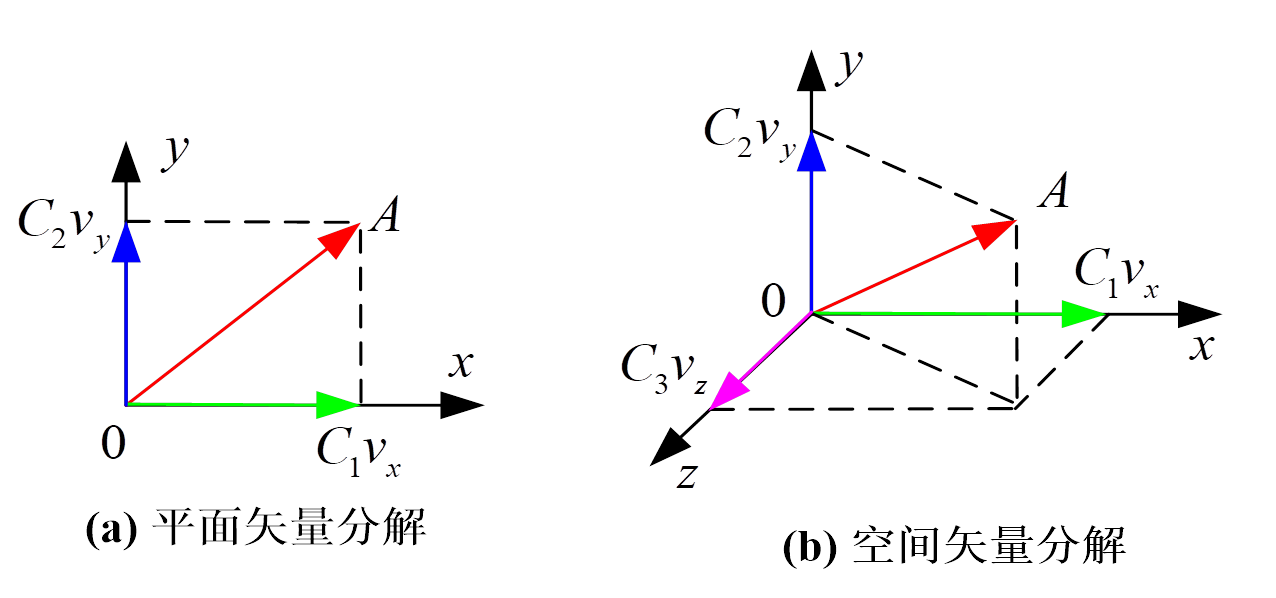
\includegraphics[scale=0.3]{vector}
\end{frame}

\begin{frame}
\begin{example}
	如三维空间中,以矢量$\bm{v_x}=(2,0,0),\bm{v_y}=(0,2,0),\bm{v_z}=(0,0,2)$所组成的集合就是一个\textbf{正交矢量集}。\\
	对于一个三维空间的矢量$\bm{A}=(2,5,8)$,可以用一个三维正交矢量集$\{v_x,v_y,v_z\}$分量的线性组合表示。即
	\[\bm{A=v_x+2.5v_y+4v_z} \]
\end{example}
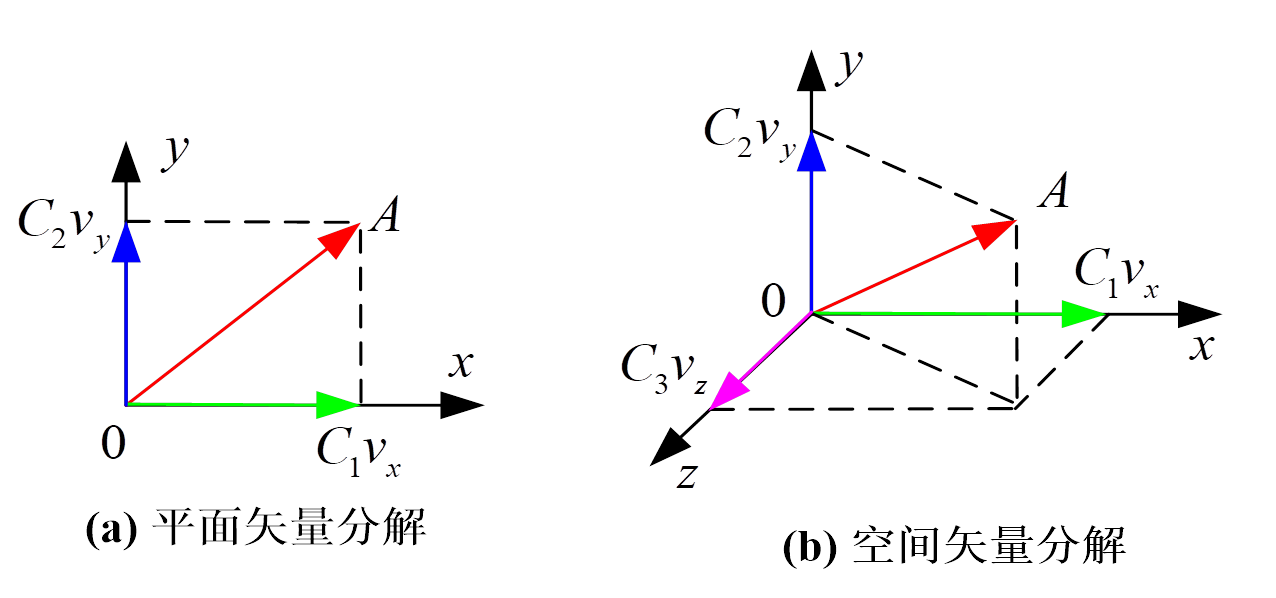
\includegraphics[scale=0.3]{vector}
\end{frame}

\begin{frame}
矢量空间正交分解的概念可推广到信号空间:在信号空间找到若干个\textbf{相互正交}的信号作为基本信号,使得信号空间中\textbf{任意信号均可表示成它们的线性组合}。 

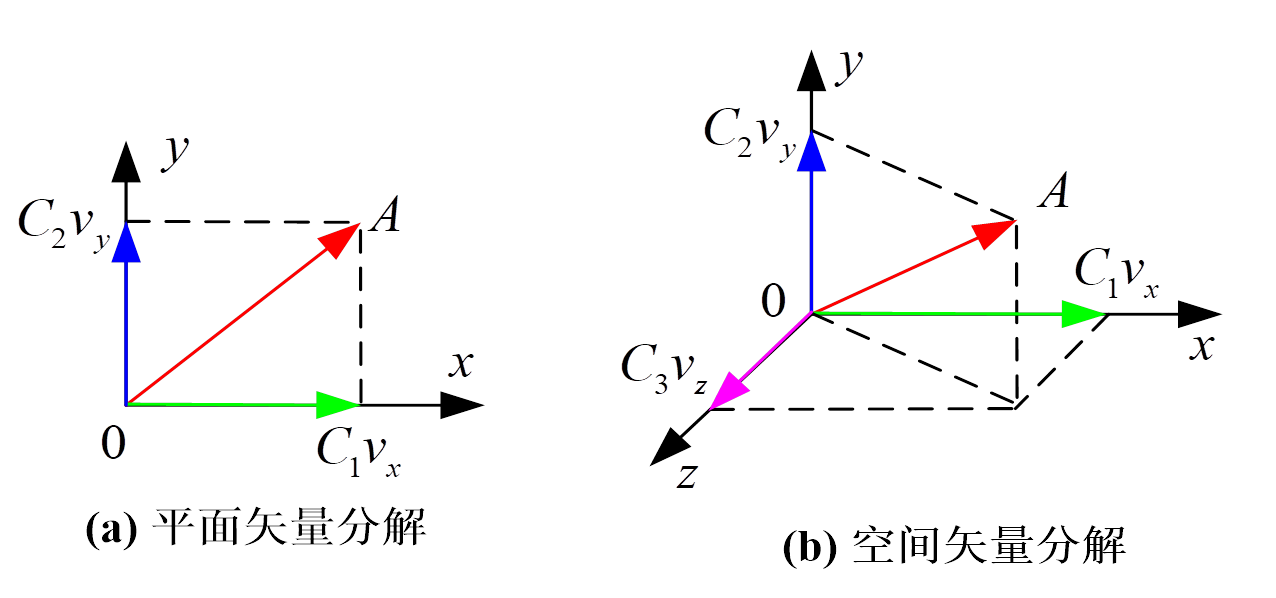
\includegraphics[scale=0.3]{vector}
\end{frame}

\begin{frame}{完备正交函数集}
三角函数集$\{1,\cos(n\omega t),\sin(n\omega t),\dots\},n=1,2,\dots$。就是在区间$(t_0,t_0,T),T=2\pi/\omega$上的完备正交函数集。
\begin{example}[傅里叶级数的三角形式]
	$f(t)=\frac{a_0}{2}+\sum\limits_{n=1}^{\infty}a_n\cos(n\omega t)+\sum\limits_{n=1}^{\infty}b_n\sin(n\omega t)$\\
	傅里叶系数: $a_n=\frac{2}{T}\int_{-\frac{T}{2}}^{\frac{T}{2}}f(t)\cos(n\omega t)dt$,\quad $b_n=\frac{2}{T}\int_{-\frac{T}{2}}^{\frac{T}{2}}f(t)\sin(n\omega t)dt$
\end{example}
\end{frame}

\begin{frame}{正交级数展开}
\begin{table}[htbp!]
\small
%\centering
\caption{正交级数展开}
\begin{tabular}{|c|c|c|c|}
	%\begin{tabular}{|p{1cm}|p{2cm}|p{2cm}|p{2cm}|}
	\hline 
	& 二维矢量 & 信号$f(t)$傅里叶展开 & 信号$x(t)$正交级数 \\ 
	\hline 
	正交集 & $\{\bm{v_x,v_y}\}$ & $\{1,\cos(n\omega t),\sin(n\omega t)\}$ & $\{f_1(t),f_2(t),\dots,f_k(t)\}$ \\ 
	\hline 
	展开系数 & $C_k=$矢量$\bm{A}$在 &
	 $a_n=\frac{2}{T}\int_{-\frac{T}{2}}^{\frac{T}{2}}f(t)\cos(n\omega t)dt$ & $x_k=\int_{0}^{T}f_k(t)x(t)dt$ \\  
	(正交投影)& 第$k$个坐标的投影&$b_n=\frac{2}{T}\int_{-\frac{T}{2}}^{\frac{T}{2}}f(t)\sin(n\omega t)dt$& $$\\ 
	\hline 
	线性表示 & $\bm{A=C_1v_x+C_2v_y}$ & $f(t)=\frac{a_0}{2}+\sum\limits_{n=1}^{\infty}a_n\cos(n\omega t)$ & $x(t)=\lim\limits_{N\to\infty}\sum\limits_{k=1}^{N}x_kf_k(t)$ \\ 
	& & $+\sum\limits_{n=1}^{\infty}b_n\sin(n\omega t)$ &  \\ 
	\hline 
\end{tabular} 
\end{table}

%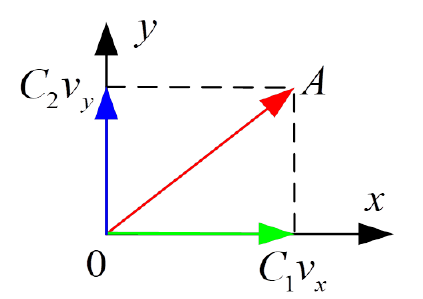
\includegraphics[scale=0.3]{vector1}
\end{frame}

\begin{frame}{确知信号的正交级数展开}
	$s(t)$是定义在(0,T)时间内的确知信号
\end{frame}

\begin{frame}{随机过程的正交级数展开}
随机过程$x(t)$展开的均方误差等于0,\\ 或者说$\lim\limits_{N\to\infty}\sum\limits_{k=1}^{N}x_kf_k(t)$均方收敛于$x(t)$
\end{frame}

\begin{frame}{随机过程的正交级数展开}
\begin{block}{Notes}
随机过程: $x(t)=\lim\limits_{N\to\infty}^N\sum\limits_{k=1}^Nx_kf_k(t)$\\
展开系数: $x_k=\int_{0}^{T}x(t)f_k(t)dt, k=1,2,\dots$\\
随机过程$x(t)$可以由上式求得的展开系数$x_k$来恢复,就是说$x(t)$完全由展开系数$x_k$确定。注意,这里对随机过程$x(t)$进行正交级数展开所用的正交函数集$\{f_k(t)\}$并没有提出特别的要求,所以\textbf{展开系数$x_k(k=1,2,\dots)$之间可能是相关的随机变量}。\\
\end{block}
\begin{block}{问题}
	如何根据噪声干扰的特性,正确选择随机过程展开的正交函数集$\{f_k\}$,以使展开系数$x_k$之间是互不相关的随机变量。
\end{block}
\end{frame}

\begin{frame}{$x_k,s_k,n_k$之间的关系}
\begin{block}{$x_k,s_k,n_k$之间的关系}
	\[x(t)=s(t)+n(t); \quad x_k=s_k+n_k \]
	随机变量$x(t)$展开系数$x_k$=确知信号$s(t)$展开系数$s_k$+噪声$n(t)$展开系数$n_k$
\end{block}
\begin{align*}
x_k&=\int_{0}^{T}f_k(t)x(t)dt\\
&=\int_{0}^{T}f_k(t)(s(t)+n(t))dt\\
&=\int_{0}^{T}f_k(t)s(t)dt+\int_{0}^{T}f_k(t)n(t))dt\\
&=s_k+n_k
\end{align*}
\end{frame}

\begin{frame}{展开系数级数展开-准备公式}
\begin{itemize}
	\item 随机过程: $x(t)=s(t)+n(t)$
	\item $\{f_k(t)\}$是一组正交函数集, $k=1,2,\dots$
	\item 随机过程$x(t)的$正交展开系数$x_k$是一个随机变量: $x_k=\int_{0}^{T}x(t)f_k(t)dt$
	\item 确知信号$s(t)$正交展开系数$s_k$是一个确定的量: $s_k=\int_{0}^{T}s(t)f_k(t)dt$
	\item 确知信号$s(t)$的展开系数$s_k$为确定的量,其均值就是本身: $E(s_k)=E\left[\int_{0}^{T}s(t)f_k(t)dt\right]=\int_{0}^{T}E[s(t)]f_k(t)dt=\int_{0}^{T}s(t)f_k(t)dt=s_k$
	\item 噪声$n(t)$是一个零均值的平稳随机过程:
	\begin{itemize}
		\item[-] $E[n(t)]=0$
		\item[-]  $n(t)$的自相关函数只取决于时间间隔$(t_k-t_j)$,而与时间的起始时刻无关,$E[n(t_j)n(t_k)]=r_n(t_k-t_j)$
	\end{itemize}
\end{itemize}
\end{frame}

\begin{frame}{展开系数$x_k$均值(推导一)}
\begin{align*}
E[x_k]&=E\left[\int_{0}^{T}f_k(t)x(t)dt\right]=E\left[\int_{0}^{T}f_k(t)(s(t)+n(t))dt\right]\\
&=E\left[\int_{0}^{T}f_k(t)s(t)dt+\int_{0}^{T}f_k(t)n(t))dt\right]\\
&=E[s_k+n_k]\\
&=E[s_k]+E[n_k]\qquad (\text{by }E[n(t)]=0\implies E[n_k]=0)\\
&= E[s_k] = s_k\qquad \text{(确知信号的展开系数为确定的量,其均值就是本身)}
\end{align*}
\end{frame}

\begin{frame}{展开系数$x_k$均值(推导二),课件采用}
\begin{align*}
E[x_k]&=E\left[\int_{0}^{T}f_k(t)x(t)dt\right]=E\left[\int_{0}^{T}f_k(t)(s(t)+n(t))dt\right]\\
&=E\left[\int_{0}^{T}f_k(t)s(t)dt+\int_{0}^{T}f_k(t)n(t))dt\right]\\
&=E\left[\int_{0}^{T}f_k(t)s(t)dt\right]+E\left[\int_{0}^{T}f_k(t)n(t))dt\right]\\
&=E\left[\int_{0}^{T}f_k(t)s(t)dt\right]+\int_{0}^{T}f_k(t)E[n(t))]dt \qquad  (\text{by }E[n(t)]=0)\\
&=E\left[\int_{0}^{T}f_k(t)s(t)dt\right]\\
&= E[s_k] = s_k\qquad \text{  (确知信号的展开系数为确定的量,其均值就是本身)}
\end{align*}
\end{frame}

\begin{frame}{展开系数$x_j$与$x_k$协方差,在t时刻两个随机变量减去各自的均值后的乘积}
\begin{align*}
&E[(x_j-E(x_j))(x_k-E(x_k))]=E[(x_j-s_j)(x_k-s_k)]\\
&=E\left[\left(\int_{0}^{T}f_j(t)x(t)dt-s_j\right)\left(\int_{0}^{T}f_k(t)x(t)dt-s_k\right)\right]\\
&=E\left[\left(\int_{0}^{T}f_j(t)(s(t)+n(t))dt-s_j\right)\left(\int_{0}^{T}f_k(t)(s(t)+n(t))dt-s_k\right)\right]\\
&=E\left[\left(\int_{0}^{T}f_j(t)n(t)dt\right)\left(\int_{0}^{T}f_k(t)n(t)dt\right)\right]=E\left[\left(\int_{0}^{T}f_j(t)n(t)dt\right)\left(\int_{0}^{T}f_k(u)n(t)du\right)\right]\\
&=E\left[\int_{0}^{T}f_j(t)\left[\int_{0}^{T}n(t)n(u)f_k(u)du\right]dt\right]=\int_{0}^{T}f_j(t)\left[\int_{0}^{T}E[n(t)n(u)]f_k(u)du\right]dt\\
&=\int_{0}^{T}f_j(t)\left[\int_{0}^{T}r_n(t-u)f_k(u)du\right]dt\quad (\text{by }E[n(t_j)n(t_k)]=r_n(t_k-t_j))
\end{align*}
\end{frame}

\begin{frame}{随机过程的卡亨南-洛维展开}
希望$x(t)$各展开系数$x_j$与$x_k$的协方差满足:
\[E[(x_j-E(x_j))(x_k-E(x_k))]=E[(x_j-s_j)(x_k-s_k)]=\lambda_k\delta_{jk} \]
式中$\delta_{jk}=
\begin{cases}
1, & (j=k)\\
0, & (j\ne k)
\end{cases}$, $\lambda_k$是展开系数$x_k$的方差, $k=1,2,\dots$\\
这样,当$j\ne k$时, $E[(x_j-s_j)(x_k-s_k)]=0$,即展开式的各展开系数之间互不相关; 当$j=k$时, $E[(x_j-s_j)(x_k-s_k)]=\lambda_k$, 是展开系数$x_k$的方差。
\end{frame}

\begin{frame}{随机过程的卡亨南-洛维展开}
展开系数$x_j$与$x_k$协方差:
\[E[(x_j-s_j)(x_k-s_k)]=\int_{0}^{T}f_j(t)\left[\int_{0}^{T}r_n(t-u)f_k(u)du\right]dt \]
其中, $x(t)=s(t)+n(t)(0\le t\le T),r_n(t-u)=E[n(t)n(u)]$是零均值平稳噪声过程$n(t)$的自相关函数。

为保证$E[(x_j-s_j)(x_k-s_k)]=\lambda_k\delta_{jk}$
\[\int_{0}^{T}r_n(t-u)f_k(u)du=\lambda_kf_k(t), 0\le t\le T \]
该式是齐次积分方程。该方程的解$f_k(t)$就是正交函数集$\{f_k(t) \}$的第$k$个坐标函数。

$E[(x_j-s_j)(x_k-s_k)]=\lambda_k\int_{0}^{T}f_j(t)f_k(t)dt=\lambda_k\delta_{jk}\implies f_j(t)$与$f_k(t)$正交。
\end{frame}

\begin{frame}{白噪声条件下正交函数集的任意性(1)}
假设接收信号为$x(t)=s(t)+n(t)$, $n(t)$是零均值,功率谱密度为$P_n(\omega)=N_0/2$的白噪声,其自相关函数为: $r_n(t-u)=\frac{N_0}{2}\delta(t-u)$,(说明噪声自相关函数在$t=u$时不为0,其他时刻都为0,自相关性最强)\\
对于任意招教函数集$\{f_k(t)\}$,展开系数$x_j$与$x_k$协方差:
\begin{align*}
E[(x_j-s_j)(x_k-s_k)]&=\int_{0}^{T}f_j(t)\left[\int_{0}^{T}r_n(t-u)f_k(u)du\right]dt\\
&=\frac{N_0}{2}\int_{0}^{T}f_j(t)\left[\int_{0}^{T}\delta(t-u)f_k(u)du\right]dt\\
&=\frac{N_0}{2}\int_{0}^{T}f_j(t)f_k(t)dt=\frac{N_0}{2}\delta_{jk}
\end{align*}
式中$\delta_{jk}=
\begin{cases}
1, & (j=k)\\
0, & (j\ne k) 
\end{cases},\quad
\delta(t-u)=
\begin{cases}
	1, & (t=u)\\
	0, & (t\ne u) 
\end{cases}
$
\end{frame}

\begin{frame}{白噪声条件下正交函数集的任意性(1)}
假设接收信号为$x(t)=s(t)+n(t)$, $n(t)$是零均值,功率谱密度为$P_n(\omega)=N_0/2$的白噪声,其自相关函数为: 
\[r_n(t-u)=\frac{N_0}{2}\delta(t-u)\]
对于任意招教函数集$\{f_k(t)\}$,展开系数$x_j$与$x_k$协方差:
\begin{align*}
E[(x_j-s_j)(x_k-s_k)]=\int_{0}^{T}f_j(t)\left[\int_{0}^{T}r_n(t-u)f_k(u)du\right]dt=\frac{N_0}{2}\delta_{jk}
\end{align*}
\begin{block}{重要结论}
	当$j\ne k$时,展开系数$x_j$与$x_k$协方差=0。这说明,在$n(t)$是白噪声的条件下,取任意正交函数集$\{f_k(t)\}$对平稳随机过程$x(t)$进行展开,其展开系数$x_k(k=1,2,\dots)$之间都是互不相关的。
	这就是白噪声条件下正交函数集的任意性。
\end{block}
\end{frame}

\begin{frame}{白噪声条件下正交函数集的任意性(2)}
\[r_n(t-u)=\frac{N_0}{2}\delta(t-u) \]
展开系数$x_j$与$x_k$协方差:
\begin{align*}
E[(x_j-s_j)(x_k-s_k)]&=\int_{0}^{T}f_j(t)\left[\int_{0}^{T}r_n(t-u)f_k(u)du\right]dt\\
&=\frac{N_0}{2}\int_{0}^{T}f_j(t)\left[\int_{0}^{T}\delta(t-u)f_k(u)du\right]dt\\
&=\frac{N_0}{2}\int_{0}^{T}f_j(t)f_k(t)dt=\frac{N_0}{2}\delta_{jk}
\end{align*}
\end{frame}

\begin{frame}{二元信号波形检测}
\tikzstyle{int}=[draw, fill=blue!20, minimum size=2em]
\begin{tikzpicture}[node distance=3.5cm,auto,>=latex']
\node [int] (a) {$x(t)$};
\node [int] (b) [right of=a] {$x_k$};
\node [int] (c) [right of=b] {$x_N$};
\node [int] (d) [below of=c] {$\frac{p(x_N|H_1)}{p(x_N|H_0)}\mathop{\gtrless}_{H_0}^{H_1}\eta$};
\node [int] (e) [left of=d] {$l(x)\mathop{\gtrless}_{H_0}^{H_1}\gamma$};
\path[->] (a) edge node {$\{f_k(t)\}$正交展开} (b);
\path[->] (b) edge node {前N项$x_k$构成$x_N$} (c);
\path[->] (c) edge [swap] node {贝叶斯检测} (d);
\path[->] (d) edge [swap] node {$N\to\infty$} (e);
\end{tikzpicture}
\end{frame}

\begin{frame}{简单二元信号波形检测}
\begin{columns}
	\column{0.4\textwidth}
	$H_0: x(t)=n(t)$\\
	$H_1: x(t)=s(t)+n(t)$\\
	$x(t)=\lim\limits_{N\to\infty}^N\sum\limits_{k=1}^Nx_kf_k(t)$\\
	$x_k=\int_{0}^{T}x(t)f_k(t)dt, k=1,2,\dots$\\
	$s_k=\int_{0}^{T}s(t)f_k(t)dt, k=1,2,\dots$\\
	$n_k=\int_{0}^{T}n(t)f_k(t)dt, k=1,2,\dots$\\
	$H_0: x_k=n_k,k=1,2,\dots$\\
	$H_1: x_k=s_k+n_k,k=1,2,\dots$
	\column{0.6\textwidth}
	\begin{itemize}
		\item 信号s(t)是确知信号,n(t)是均值为0,功率谱密度为$P_n(\omega)=N_0/2$的高斯白噪声;
		\item 无论在假设$H_1$下还是在假设$H_2$下,接收信号的$x(t)$都是高斯随机过程;
		\item 展开系数$x_k$是高斯随机过程的积分结果,因而$x_k$是高斯随机变量;
		\item 展开系数$x_k$之间是互不相关的,也是相互统计独立的;
		\item 高斯随机变量由均值和方差决定。由此求出两个假设下的概率密度函数$p(x_k|H_j),k=1,2,\dots;j=0,1$。
	\end{itemize}
\end{columns}
\end{frame}

\begin{frame}{简单二元信号波形检测$H_0$}
$n(t)$是高斯白噪声$\implies E[n(t)n(u)]=r_n(t-u) =\frac{N_0}{2}\delta(t-u)=\frac{N_0}{2},(\delta(t-u)=1,t=u)$ \\
$f_k(t)$是一组正交函数集$\implies\int_{0}^{T}f_j(t)f_k(t)dt=1,(j=k)$
\begin{align*}
Var[x_k|H_0]&=E[n_k^2]=E\left[\int_{0}^{T}n(t)f_k(t)dt\int_{0}^{T}n(u)f_k(u)du\right]\\
&=\int_{0}^{T}f_k(t)\left\{\int_{0}^{T}E[n(t)n(u)]f_k(u)du\right\}dt\\
&=\int_{0}^{T}f_k(t)\left[\int_{0}^{T}\frac{N_0}{2}\delta(t-u)f_k(u)du\right]dt\\
&=\int_{0}^{T}f_k(t)\frac{N_0}{2}f_k(t)dt\\
&=\frac{N_0}{2}
\end{align*}
\end{frame}

\begin{frame}{简单二元信号波形检测$H_1$}
$x_k=\int_{0}^{T}x(t)dt=\int_{0}^{T}[s(t)+n(t)]dt=\int_{0}^{T}s(t)dt+\int_{0}^{T}n(t)dt=s_k+n_k$\\
$x_k=s_k+n_k$
\begin{align*}
E[x_k|H_1]&=E[s_k+n_k]&\text{by }x_k=s_k+n_k \\
&=E(s_k)+E(n_k)&\text{by }E(n_k)=0 \\
&=E(s_k)=s_k&\text{(确知信号展开系数为确定量,其均值就是本身)}\\
Var[x_k|H_1]&=E[(x_k-E[x_k])^2]&\text{by }x_k=s_k+n_k,E[x_k]=s_k\\
&=E[(s_k+n_k-s_k)^2]&\\
&=E[n_k^2]=\frac{N_0}{2}&
\end{align*}
或: $E[x_k|H_1]=E\left[\int_{0}^{T}x(t)f_k(t)dt\right]=E\left[\int_{0}^{T}(s(t)+n(t))f_k(t)dt\right]$\\
$=E\left[\int_{0}^{T}s(t)dt\right]+\int_{0}^{t}E[n(t)])f_k(t)dt=E\left[\int_{0}^{T}s(t)dt\right]=E[s_k]=s_k$
\end{frame}

\begin{frame}{简单二元信号波形检测-判决式预备公式}
\[\ln\lambda(\bm{x}_N)=\frac{p(\bm{x}_N|H_1)}{p(\bm{x}_N|H_0)}=\frac{2}{N_0}\sum\limits_{k=1}^{N}x_ks_k-\frac{1}{N_0}\sum\limits_{k=1}^{N}s_k^2\mathop{\gtrless}_{H_0}^{H_1}\ln\eta \]
\begin{align*}
&x(t)=\lim\limits_{N\to\infty}\sum\limits_{k=1}^Nx_kf_k(t)\\
&x_k=\int_{0}^{T}x(t)f_k(t)dt, k=1,2,\dots\\
&s(t)=\lim\limits_{N\to\infty}\sum\limits_{k=1}^Ns_kf_k(t)\\
&s_k=\int_{0}^{T}s(t)f_k(t)dt, k=1,2,\dots\\
&E_s=\int_{0}^{T}s^2(t)dt
\end{align*}
\end{frame}

\begin{frame}{简单二元信号波形检测-判决式推导(1)}
\begin{align*}
\lim\limits_{N\to\infty}\sum\limits_{k=1}^{N}x_ks_k&=\left[\lim\limits_{N\to\infty}\sum\limits_{k=1}^{N}x_k\right]s_k\\
&=\left[\lim\limits_{N\to\infty}\sum\limits_{k=1}^{N}x_k\right]\int_{0}^{T}s(t)f_k(t)dt\\
&=\int_{0}^{T}s(t)\left[\lim\limits_{N\to\infty}\sum\limits_{k=1}^{N}x_kf_k(t)\right]dt\\
&=\int_{0}^{T}s(t)x(t)dt
\end{align*}
\end{frame}

\begin{frame}{简单二元信号波形检测-判决式推导(2)}
\begin{align*}
\lim\limits_{N\to\infty}\sum\limits_{k=1}^{N}s_k^2&=\left[\lim\limits_{N\to\infty}\sum\limits_{k=1}^{N}s_k\right]s_k\\
&=\left[\lim\limits_{N\to\infty}\sum\limits_{k=1}^{N}s_k\right]\int_{0}^{T}s(t)f_k(t)dt\\
&=\int_{0}^{T}s(t)\left[\lim\limits_{N\to\infty}\sum\limits_{k=1}^{N}s_kf_k(t)\right]dt\\
&=\int_{0}^{T}s(t)s(t)dt=\int_{0}^{T}s^2(t)dt=E_s
\end{align*}
\end{frame}

\begin{frame}{简单二元信号波形检测-检测性能(1)}
\textbf{判决表达式:}
\[l[x(t)]\mathop{=}^{def}\int_{0}^{T}x(t)s(t)dt\mathop{\gtrless}_{H_0}^{H_1}\frac{N_0}{2}\ln\eta+\frac{E_s}{2}\mathop{=}^{def}\gamma \]
检验统计量$l[x(t)]$无论在假设$H_0$下,还是在假设$H_1$下,都是由高斯随机过程$x(t)s(t)(0\le t\le T)$经积分得到的,所以\bm{$l[x(t)]$}\textbf{是高斯随机变量}。
\begin{enumerate}
	\item 求出检验统计量$l[x(t)]$在两个假设下的均值$E(l|H_j)$和方差$Var(l|H_j),j=0,1$;
	\item 求各种判决概率$P(H_i|H_j),i,j=0,1$;\\
	简单二元信号检测与雷达信号检测相对应:$P(H_1|H_0)\mathop{=}\limits^{def}P_F$(称为虚警概率),$P(H_1|H_1)\mathop{=}\limits^{def}P_D$(称为检测概率)
	\item 计算检测性能。
\end{enumerate}
\end{frame}

\begin{frame}{简单二元信号波形检测-检测性能(2)}
\begin{enumerate}[1]
	\item 定义统计量:$l\mathop{=}\limits^{def}\int_{0}^{T}x(t)s(t)dt$
	\item 假设$H_0,H_1$下检验统计量$l[x(t)]$的均值和方差分别为\\
	$E[l|H_0]=E\left[\int_{0}^{T}x(t)s(t)dt|H_0\right]=E\left[\int_{0}^{T}n(t)s(t)dt\right]=0$\\ 
	$Var[l|H_0]=E[((l|H_0)-E(l|H_0))^2]=\frac{N_0}{2}E_s$\\
	$E[l|H_1]=E\left[\int_{0}^{T}x(t)s(t)dt|H_1\right]=E\left[\int_{0}^{T}(s(t)+n(t))s(t)dt\right]=E_s$\\
	$Var[l|H_1]=E[((l|H_1)-E(l|H_1))^2]=\frac{N_0}{2}E_s$\\
	\item 假设$H_0,H_1$下服从高斯分布的检验统计量$l[x(t)]$的概率密度函数分别为\\
\[p(l|H_0)=\left(\frac{1}{\pi N_0E_s}\right)^{1/2}\exp\left(-\frac{l^2}{N_0E_s}\right)\]
	\[p(l|H_1)=\left(\frac{1}{\pi N_0E_s}\right)^{1/2}\exp\left(-\frac{(l-E_s)^2}{N_0E_s}\right)\]
\end{enumerate}
\end{frame}
\begin{frame}{简单二元信号波形检测-检测性能(3)}
\begin{enumerate}
	\setcounter{enumi}{3} 
	\item 求各种判决概率$P(H_i|H_j),i,j=0,1$\\
	虚警概率:$P(H_1|H_0)\mathop{=}\limits^{def}P_F=Q\left[\frac{\ln\eta}{d}+\frac{d}{2}\right]$\\ 检测概率:$P(H_1|H_1)\mathop{=}\limits^{def}P_D=Q\left[\frac{\ln\eta}{d}-\frac{d}{2}\right]$\\
	$P(H_0|H_1)=1-P(H_1|H_1)=1-Q\left[\frac{\ln\eta}{d}-\frac{d}{2}\right]$\\
	$P(H_0|H_0)=1-P(H_1|H_0)=1-Q\left[\frac{\ln\eta}{d}+\frac{d}{2}\right]$\\
	$d^2\mathop{=}\limits^{def}\frac{(E(l|H_1)-E(l|H_0))^2}{Var(l|H_0)}=\frac{2E_s}{N_0}$ \qquad 偏移系数$d^2$表示功率信噪比\\
\end{enumerate}
\begin{block}{结论}
	对简单二元信号来讲,只要保持确知信号$s(t)$的能量不变,信号波形可以任意设计,检测性能不发生变化。
\end{block}
\end{frame}

\begin{frame}{计算$E[l|H_0]$}
\begin{align*}
E[l|H_0]&=E\left[\int_{0}^{T}x(t)s(t)dt|H_0\right] &\text{by }H_0: x(t)=n(t)\\
&=E\left[\int_{0}^{T}n(t)s(t)dt\right]&\\
&=\int_{0}^{T}E[n(t)]s(t)dt=0 &\text{by }E[n(t)]=0
\end{align*}
\end{frame}

\begin{frame}{计算$Var[l|H_0]$}
$H_0:x(t)=n(t), E(l|H_0)=0,E_s=\int_{0}^{T}s^2(t)dt$\\
$E[n(t)n(u)]=r_n(t-u)=\frac{N_0}{2}\delta(t-u)=\frac{N_0}{2},(t=u,\delta(t-u)=1)$
\begin{align*}
Var[l|H_0]&=E[((l|H_0)-E(l|H_0))^2]=E[(l|H_0)^2]=E\left[\left(\int_{0}^{T}x(t)s(t)dt\right)^2\right]\\
&=E\left[\int_{0}^{T}n(t)s(t)dt\int_{0}^{T}n(t)s(t)dt\right]=E\left[\int_{0}^{T}n(t)s(t)dt\int_{0}^{T}n(u)s(u)du\right]\\
&=\int_{0}^{T}s(t)\left\{\int_{0}^{T}E[n(u)n(t)]s(u)du\right\}dt=\int_{0}^{T}s(t)\left[\int_{0}^{T}\frac{N_0}{2}\delta(t-u)s(u)du\right]dt\\
&=\frac{N_0}{2}\int_{0}^{T}s(t)\left(\int_{0}^{T}s(u)du\right)dt=\frac{N_0}{2}\int_{0}^{T}s^2(t)dt\\
&=\frac{N_0}{2}E_s
\end{align*}
\end{frame}

\begin{frame}{计算$p(l|H_0)$}
$E[l|H_0]=0,Var[l|H_0]=\frac{N_0}{2}E_s$
\begin{align*}
p(l|H_0)&=\left(\frac{1}{2\pi Var[l|H_0]}\right)^{1/2}\exp\left(-\frac{(l-E[l|H_0])^2}{2Var[l|H_0]}\right)\\
&=\frac{1}{\sqrt{\pi N_0E_s}}\exp\left(-\frac{l^2}{N_0E_s}\right)
\end{align*}
\end{frame}

\begin{frame}{计算$E[l|H_1]$}
\begin{align*}
E[l|H_1]&=E\left[\int_{0}^{T}x(t)s(t)dt|H_1\right] &\text{by }H_1: x(t)=s(t)+n(t)\\
&=E\left[\int_{0}^{T}(s(t)+n(t))s(t)dt\right]&\\
&=E\left[\int_{0}^{T}s^2(t)dt\right]+\int_{0}^{T}E[n(t)]s(t)dt& \text{by } E[n(t)]=0 \\
&=E\left[\int_{0}^{T}s^2(t)dt\right]& \text{by } E_s=\int_{0}^{T}s^2(t)dt 
&=E_s
\end{align*}
\end{frame}

\begin{frame}{计算$Var[l|H_1]$}
$H_1:x(t)=s(t)+n(t), E(l|H_1)=E_s,E_s=\int_{0}^{T}s^2(t)dt$\\
$E[n(t)n(u)]=r_n(t-u)=\frac{N_0}{2}\delta(t-u)=\frac{N_0}{2},(t=u,\delta(t-u)=1)$
\begin{align*}
Var[l|H_1]&=E[((l|H_1)-E(l|H_1))^2]=E\left[\left(\int_{0}^{T}(s(t)+n(t))s(t)dt-E_s\right)^2\right]\\
&=E\left[\left(\int_{0}^{T}(s^2(t)dt+\int_{0}^{T}n(t)s(t)dt-E_s\right)^2\right]=E\left[\left(\int_{0}^{T}n(t)s(t)dt\right)^2\right]\\
&=E\left[\int_{0}^{T}n(t)s(t)dt\int_{0}^{T}n(t)s(t)dt\right]=E\left[\int_{0}^{T}n(t)s(t)dt\int_{0}^{T}n(u)s(u)du\right]\\
&=\int_{0}^{T}s(t)\left\{\int_{0}^{T}E[n(u)n(t)]s(u)du\right\}dt=\int_{0}^{T}s(t)\left[\int_{0}^{T}\frac{N_0}{2}\delta(t-u)s(u)du\right]dt\\
&=\frac{N_0}{2}\int_{0}^{T}s(t)\left(\int_{0}^{T}s(u)du\right)dt=\frac{N_0}{2}\int_{0}^{T}s^2(t)dt=\frac{N_0}{2}E_s
\end{align*}
\end{frame}

\begin{frame}{计算$p(l|H_1)$}
$E[l|H_1]=E_s,Var[l|H_1]=\frac{N_0}{2}E_s$
\begin{align*}
p(l|H_1)&=\left(\frac{1}{2\pi Var[l|H_1]}\right)^{1/2}\exp\left(-\frac{(l-E[l|H_1])^2}{2Var[l|H_1]}\right)\\
&=\frac{1}{\sqrt{\pi N_0E_s}}\exp\left(-\frac{(l-E_s)^2}{N_0E_s}\right)
\end{align*}
\end{frame}

\begin{frame}{计算$P(H_1|H_0)$}
\begin{align*}
P(H_1|H_0)&\mathop{=}^{def}P_F=\int_{\gamma}^{\infty}p(l|H_0)dl\\
&=\int_{\gamma}^{\infty}\left(\frac{1}{\pi N_0E_s}\right)^{1/2}\exp\left(-\frac{l^2}{N_0E_s}\right)dl\\
&\mathop{=}^{u=\frac{l}{\sqrt{N_0E_s/2}}}\int_{\frac{\gamma}{\sqrt{N_0E_s/2}}}^{\infty}\left(\frac{1}{2\pi}\right)^{1/2}\exp\left(-\frac{u^2}{2}\right)du\\
&=Q\left[\frac{\gamma}{\sqrt{N_0E_s/2}}\right]\mathop{=}^{\gamma=\frac{N_0}{2}\ln\eta+\frac{E_s}{2}}Q\left[\frac{\frac{N_0}{2}\ln\eta+\frac{E_s}{2}}{\sqrt{N_0E_s/2}}\right]\\
&=Q\left[\frac{\ln\eta}{d}+\frac{d}{2}\right]\qquad d^2=\frac{2E_s}{N_0}
\end{align*}
偏移系数$d^2$表示功率信噪比。
\end{frame}

\begin{frame}{计算$P(H_0|H_1)$}
\begin{align*}
P(H_1|H_1)&\mathop{=}^{def}P_D=\int_{\gamma}^{\infty}p(l|H_1)dl\\
&=\int_{\gamma}^{\infty}\left(\frac{1}{\pi N_0E_s}\right)^{1/2}\exp\left(-\frac{(l-E_s)^2}{N_0E_s}\right)dl\\
&\mathop{=}^{u=\frac{l-E_s}{\sqrt{N_0E_s/2}}}\int_{\frac{\gamma-E_s}{\sqrt{N_0E_s/2}}}^{\infty}\left(\frac{1}{2\pi}\right)^{1/2}\exp\left(-\frac{u^2}{2}\right)du\\
&=Q\left[\frac{\gamma-E_s}{\sqrt{N_0E_s/2}}\right]\mathop{=}^{\gamma=\frac{N_0}{2}\ln\eta+\frac{E_s}{2}}Q\left[\frac{\frac{N_0}{2}\ln\eta-\frac{E_s}{2}}{\sqrt{N_0E_s/2}}\right]\\
&=Q\left[\frac{\ln\eta}{d}-\frac{d}{2}\right]\qquad d^2=\frac{2E_s}{N_0}
\end{align*}
偏移系数$d^2$表示功率信噪比。
\end{frame}

\section{简单二元信号波形的检测-充分统计量方法}

\begin{frame}{充分量统计法,巧取$f_1(t)$}
相互正交的函数集$\{f_k(t)\}(k=1,2,\dots)\implies$
$\int_{0}^{T}f_j(t)f_k(t)dt=
\begin{cases}
1,&j=k\\
0,&j\ne k
\end{cases}
$\\
设$f_1(t)=\frac{1}{\sqrt{E_s}}s(t)\implies s(t)=\sqrt{E_s}f_1(t)$\\
由于$f_1(t)$与$f_k(t)(k\ge 2)$正交$\implies s(t)$与$f_k(t)(k\ge 2)$正交\\
$\implies$确知信号$s(t)$在$f_k(t)(k\ge 2)$上的投影等于0,即$s_k=0,(k\ge 2)$\\
$s_k=\int_{0}^{T}s(t)f_k(t)dt=\int_{0}^{T}\sqrt{E_s}f_1(t)f_k(t)dt=\sqrt{E_s}f_1(t)f_k(t)$\\
$k=1,\quad f_1(t)f_k(t)=1\implies s_1=\sqrt{E_s};\qquad k\ge 2,\quad f_1(t)f_k(t)=0\implies s_k=0$\\
进一步,由于$x(t)=s(t)+n(t),\quad x_k=s_k+n_k,\quad n(t)$是高斯白噪声过程。\\
\begin{block}{结论}
	$x_1=s_1+n_1=\sqrt{E_s}+n_1\implies x_1$是高斯随机变量。含有确知信号$s(t)$信息。\\
	$x_k=s_k+n_k=n_k\quad(k\ge 2)\implies x_k(k\ge 2)$是高斯随机变量,且相互统计独立。不含确知信号$s(t)$信息,对判决没有影响。\\
\end{block}
\end{frame}

\begin{frame}{充分量统计法(1)}
(2)利用构造的正交函数集$f_1(t)$和$\{f_k(t)|k\ge 2\}$,对接收信号进行正交展开
\begin{block}{假设$H_0:x(t)=n(t)$下,展开系数}	
	$x_1=\int_{0}^{T}x(t)f_1(t)dt=\int_{0}^{T}n(t)f_1(t)dt=n_1$\\
	
	$x_k=\int_{0}^{T}x(t)f_k(t)dt=\int_{0}^{T}n(t)f_k(t)dt=n_k\qquad k\ge 2$
\end{block}
\begin{block}{假设$H_1:x(t)=s(t)+n(t)$下,展开系数}
	$x_1=\int_{0}^{T}x(t)f_1(t)dt=\int_{0}^{T}[s(t)+n(t)]f_1(t)dt=\int_{0}^{T}s(t)f_1(t)dt+\int_{0}^{T}n(t)f_1(t)dt$\\
	$=\int_{0}^{T}s(t)[\frac{1}{\sqrt{E_s}}s(t)]dt+n_1=\frac{1}{\sqrt{E_s}}\int_{0}^{T}s^2(t)dt+n_1$\\
	$=\sqrt{E_s}+n_1\qquad (\text{by }f_1(t)=\frac{1}{\sqrt{E_s}}s(t),E_s=\int_{0}^{T}s^2(t)dt)$\\
	
	$x_k=\int_{0}^{T}x(t)f_k(t)dt=\int_{0}^{T}[s(t)+n(t)]f_k(t)dt=\int_{0}^{T}[\sqrt{E_s}f_1(t)+n(t)]f_k(t)dt$\\
	$=\int_{0}^{T}n(t)f_k(t)dt=n_k\qquad k\ge 2$\qquad (by\quad $s(t)=\sqrt{E_s}f_1(t), \int_{0}^{T}f_1(t)f_k(t)dt=0,k\ge 2$)
\end{block}
\end{frame}

\begin{frame}{充分量统计法(2)}
(2)利用构造的正交函数集$f_1(t)$和$\{f_k(t)|k\ge 2\}$,对接收信号进行正交展开
\begin{block}{假设$H_0:x(t)=n(t)$下,展开系数}	
	$x_1=\int_{0}^{T}x(t)f_1(t)dt=\int_{0}^{T}n(t)f_1(t)dt=n_1\implies$不含接收信号信息\\
	
	$x_k=\int_{0}^{T}x(t)f_k(t)dt=\int_{0}^{T}n(t)f_k(t)dt=n_k\qquad k\ge 2$
\end{block}
\begin{block}{假设$H_1:x(t)=s(t)+n(t)$下,展开系数}
	$x_1=\int_{0}^{T}x(t)f_1(t)dt=\int_{0}^{T}[s(t)+n(t)]f_1(t)dt=\sqrt{E_s}+n_1\implies x_1$是高斯随机变量,含有接收信号/确知信号$s(t)$信息 \\
	$x_k=\int_{0}^{T}x(t)f_k(t)dt=\int_{0}^{T}[s(t)+n(t)]f_k(t)dt=n_k\qquad k\ge 2\implies x_k$是高斯随机变量,且相互统计独立。但不含有接收信号/确知信号$s(t)$信息 \\
\end{block}
\begin{block}{通过两个假设下的展开系数$x_1$即可判定假设$H_1$为真,还是$H_0$为真。}
\end{block}
\end{frame}


\begin{frame}{充分量统计法,接收信号$x_1(t)$}
因为$f_1(t)=\frac{1}{\sqrt{E_s}}s(t),x_1|H_0=n_1,x_1|H_1=\sqrt{E_s}+n_1$\\ $x_1=\int_{0}^{T}x(t)f_1(t)dt=\frac{1}{\sqrt{E_s}}\int_{0}^{T}x(t)s(t)dt$\\
所以充分统计量$x_1$是高斯随机变量,可用假设$H_0$和假设$H_1$下的均值和方差表示。
\end{frame}

\begin{frame}{充分量统计法,判决表达式}
\textbf{判决表达式:}
\[l[x(t)]\mathop{=}^{def}\int_{0}^{T}x(t)s(t)dt\mathop{\gtrless}_{H_0}^{H_1}\frac{N_0}{2}\ln\eta+\frac{E_s}{2}\mathop{=}^{def}\gamma \]
~\\
\begin{block}{结论}
由任意正交函数集对$x(t)$进行正交级数展开法与由充分统计量法导出的判决表达式是完全一样的,因而也具有相同的检测系统结构和相同的检测性能。
\end{block}
\end{frame}

\begin{frame}{推导$E[x_1|H_0]$}
$f_1(t)=\frac{1}{\sqrt{E_s}}s(t),x_1|H_0=n_1,x_1|H_1=\sqrt{E_s}+n_1$\\ $x_1=\int_{0}^{T}x(t)f_1(t)dt=\frac{1}{\sqrt{E_s}}\int_{0}^{T}x(t)s(t)dt$\\
$E[x_1|H_0]=E[n_1]=0$\\
或:
\begin{align*}
E[x_1|H_0]&=E\left[\frac{1}{\sqrt{E_s}}\int_{0}^{T}x(t)s(t)dt\right] &\text{by }H_0: x(t)=n(t)\\
&=E\left[\frac{1}{\sqrt{E_s}}\int_{0}^{T}n(t)s(t)dt\right]&\\
&=\frac{1}{\sqrt{E_s}}\int_{0}^{T}E[n(t)]s(t)dt=0 &\text{by }E[n(t)]=0
\end{align*}
\end{frame}

\begin{frame}{推导$Vax[x_1|H_0]$(方法1)}
$H_0:x(t)=n(t), E(x_1|H_0)=0,E_s=\int_{0}^{T}s^2(t)dt$\\
$E[n(t)n(u)]=r_n(t-u)=\frac{N_0}{2}\delta(t-u)=\frac{N_0}{2},(t=u,\delta(t-u)=1)$\\
$f_1(t)=\frac{1}{\sqrt{E_s}}s(t),x_1|H_0=n_1,x_1|H_1=\sqrt{E_s}+n_1$\\ $x_1=\int_{0}^{T}x(t)f_1(t)dt=\frac{1}{\sqrt{E_s}}\int_{0}^{T}x(t)s(t)dt,x_1|H_0=\frac{1}{\sqrt{E_s}}\int_{0}^{T}n(t)s(t)dt$
\begin{align*}
&Var[x_1|H_0]=E[((x_1|H_0)-E(x_1|H_0))^2]=E[(x_1|H_0)^2]=E\left[\left(\frac{1}{\sqrt{E_s}}\int_{0}^{T}n(t)s(t)dt\right)^2\right]\\
&=\frac{1}{E_s}E\left[\int_{0}^{T}n(t)s(t)dt\int_{0}^{T}n(t)s(t)dt\right]=\frac{1}{E_s}E\left[\int_{0}^{T}n(t)s(t)dt\int_{0}^{T}n(u)s(u)du\right]\\
&=\frac{1}{E_s}\int_{0}^{T}s(t)\left\{\int_{0}^{T}E[n(u)n(t)]s(u)du\right\}dt=\frac{1}{E_s}\int_{0}^{T}s(t)\left[\int_{0}^{T}\frac{N_0}{2}\delta(t-u)s(u)du\right]dt\\
&=\frac{N_0}{2E_s}\int_{0}^{T}s(t)\left(\int_{0}^{T}s(u)du\right)dt=\frac{N_0}{2E_s}\int_{0}^{T}s^2(t)dt=\frac{N_0}{2}
\end{align*}
\end{frame}

\begin{frame}{推导$Vax[x_1|H_0]$(方法2)}
$H_0:x(t)=n(t), E(x_1|H_0)=0,E_s=\int_{0}^{T}s^2(t)dt$\\
$E[n(t)n(u)]=r_n(t-u)=\frac{N_0}{2}\delta(t-u)=\frac{N_0}{2},(t=u,\delta(t-u)=1)$\\
$f_1(t)=\frac{1}{\sqrt{E_s}}s(t),x_1|H_0=n_1,x_1|H_1=\sqrt{E_s}+n_1$\\ $x_1=\int_{0}^{T}x(t)f_1(t)dt=\frac{1}{\sqrt{E_s}}\int_{0}^{T}x(t)s(t)dt,x_1|H_0=\frac{1}{\sqrt{E_s}}\int_{0}^{T}n(t)s(t)dt$
$n_1=\int_{0}^{T}n(t)f_1(t)dt=\int_{0}^{T}n(t)\frac{1}{\sqrt{E_s}}s(t)dt=\frac{1}{\sqrt{E_s}}\int_{0}^{T}n(t)s(t)dt$
\begin{align*}
Var[x_1|H_0]&=E[((x_1|H_0)-E(x_1|H_0))^2]=E[(x_1|H_0)^2]=E[n_1^2]\\
&=E\left[\left(\frac{1}{\sqrt{E_s}}\int_{0}^{T}n(t)s(t)dt\right)^2\right]\qquad (\text{以下同方法1})\\
&=\frac{N_0}{2}
\end{align*}
\end{frame}

\begin{frame}{推导$p(x_1|H_0)$}
$E[x_1|H_0]=0,Var[x_1|H_0]=\frac{N_0}{2}$
\begin{align*}
p(x_1|H_0)&=\left(\frac{1}{2\pi Var[x_1|H_0]}\right)^{1/2}\exp\left(-\frac{(x_1-E[x_1|H_0])^2}{2Var[x_1|H_0]}\right)\\
&=\frac{1}{\sqrt{\pi N_0}}\exp\left(-\frac{x_1^2}{N_0}\right)
\end{align*}
\end{frame}

\begin{frame}{推导$E[x_1|H_1]$}
$x_1|H_1=\sqrt{E_s}+n_1$
\begin{align*}
E[x|H_1]&=E\left[\sqrt{E_s}+n_1\right]\\
&=E[\sqrt{E_s}]+E[n_1]\\
&=E[\sqrt{E_s}]=\sqrt{E_s}
\end{align*}
\end{frame}

\begin{frame}{推导$Var[x_1|H_1]$}
$x_1|H_1=\sqrt{E_s}+n_1,E(x_1|H_1)=\sqrt{E_s}$
\begin{align*}
Var[x|H_1]&=E[((x|H_1)-E(x|H_1))^2]=E[n_1^2]\\
&=Var[x_1|H_0]\\
&=\frac{N_0}{2}
\end{align*}
\end{frame}

\begin{frame}{推导$p(x_1|H_1)$}
$E[x_1|H_1]=\sqrt{E_s},Var[x_|H_1]=\frac{N_0}{2}$
\begin{align*}
p(x_1|H_1)&=\left(\frac{1}{2\pi Var[x_1|H_1]}\right)^{1/2}\exp\left(-\frac{(x_1-E[x_1|H_1])^2}{2Var[x_1|H_1]}\right)\\
&=\frac{1}{\sqrt{\pi N_0}}\exp\left(-\frac{(x_1-\sqrt{E_s})^2}{N_0}\right)
\end{align*}
\end{frame}

\section{一般二元信号波形检测}

\begin{frame}{最佳信号波形设计}
波形相关系数: $\rho\mathop{=}\limits^{def}\frac{1}{\sqrt{E_{0}E_{1}}}\int_{0}^{T}s_0(t)s_1(t)dt,\quad(|\rho|\le 1)$\\
~\\
偏移系数: $d^2\mathop{=}\limits^{def}\frac{(E(l|H_1)-E(l|H_0))^2}{Var(l|H_0)}=\frac{2}{N_0}(E_1+E_0-2\rho\sqrt{E_1E_0})$
\begin{block}{最检波形设计$\rho=-1,s_0(t)=-s_1(t),d^2=\frac{8}{N_0}E_s,E_0=E_1=E_s$}
	在高斯白噪声条件下,对于确知一般二元信号的波形检测,当两个信号设计成互反信号时,可在信号能量给定的约束下获得最好的检测性能。
\end{block}
\begin{block}{正交波形设计$\rho=0,d^2=\frac{4}{N_0}E_s,E_0=E_1=E_s$}
	信号的检测性能差于同信号能量的反相信号。
\end{block}
\begin{block}{不合理波形设计$0<\rho\le 1,E_0=E_1=E_s$}
	$\frac{4}{N_0}E_s>d^2\ge 0\implies\rho\to 1,d^2\to 0$,检测性能逐步变差。
\end{block}
\end{frame}

\begin{frame}{检测性能}
\begin{block}{}
	简单二元信号,检测性能与$d^2$有关; 一般二元信号,检测性能不但与$d^2$有关,还与相关系数$\rho$有关,$\rho=-1$时,可获得最佳性能。
\end{block}
\end{frame}

\section{课件公式}

\begin{frame}{积分}
\[\int \sin^2(x)dx=\frac{x}{2}-\frac{1}{4}sin(2x)+C\]
\[\int_{0}^{T}a^2\sin^2(\omega t)dt=\frac{a^2T}{2}, T=2\pi/\omega\]
\begin{align*}
E_s&=\int_{0}^{T}s^2(t)dt\\
&=\int_{0}^{2\pi}(5\sin(t))^2dt\\
&=25\pi
\end{align*}
\[s(t)=\lim\limits_{N\to \infty}\sum_{1}^{N}s_kf_k(t)\]
\end{frame}

\begin{frame}{$E[n(t)n(u)]$}
$E[n(t)n(u)]=r_n(t-u)=\frac{N_0}{2}\delta(t-u)=\frac{N_0}{2},(t=u,\delta(t-u)=1)$\\
~\\
$E[n(t)n(u)]=\frac{N_0}{2}$\\
~\\
白噪声功率谱密度$P_n(\omega)=\frac{N_0}{2},(N_0$是常数)
\end{frame}

\begin{frame}{$\delta_{jk}$}
$\delta_{jk}=
\begin{cases}
1, & (j=k)\\
0, & (j\ne k)
\end{cases}
$, $k=1,2,\dots$
\end{frame}

\begin{frame}{积分均值互换推导}
\begin{align*}
\mu_x(t)&\mathop{=}^{def}E[x(t)]=\int_{-\infty}^{\infty}xp(x;t)dx&\\
E[\int_{0}^{T}x(t)f_k(t)dt]&=\int_{-\infty}^{\infty}\int_{0}^{T}x(t)f_k(t)dtp(x;t)dx\\
&=\int_{0}^{T}\int_{-\infty}^{\infty}x(t)f_k(t)p(x;t)dxdt\\
&=\int_{0}^{T}\left(\int_{-\infty}^{\infty}x(t)p(x;t)dx\right)f_k(t)dt\\
&=\int_{0}^{T}E[x(t)]f_k(t)dt
\end{align*}
\end{frame}

\begin{frame}{$E_{s_0}+E_{s_1}=2E_s$}
若两个正数之和为$\alpha$常数,则当这两个正数各为$\alpha/2$时其乘积最大。
\end{frame}

\begin{frame}{正交}
\begin{theorem}
	组成三角级数的函数系$\{1,\cos x,\sin x,\cos 2x,\sin 2x,\dots,\cos nx,\sin nx,\dots \}$在$[-\pi,\pi]$上正交,即其中任意两个不同的函数之积在$[-\pi,pi]$上的积分等于0.
\end{theorem}
\begin{proof}
	\begin{align*}
	&\int_{-\pi}^{\pi}1\cdot\cos nxdx=\int_{-\pi}^{\pi}1\cdot\sin nxdx=0\quad (n=1,2,\dots)\\
	&\int_{-\pi}^{\pi}\cos kx\cos nxdx=\frac{1}{2}\int_{-\pi}^{\pi}[\cos(k+n)x+cos(k-n)x]dx=0\quad (k\ne n)\\
	&\text{同理可证:}\\
	&\int_{-\pi}^{\pi}\sin kx\sin nxdx=0, \int_{-\pi}^{\pi}\cos kx\sin nxdx=0\quad (k\ne n)\\
	\end{align*}
\end{proof}
\end{frame}

\begin{frame}{temp}
$5\sin(2t)$\\
~\\
$n(t)$\\
~\\
$x(t)$\\
~\\
$\int_{0}^{T}s_{1}(t)x(t)dt$\\
~\\
$\int_{0}^{T}s_{0}(t)x(t)dt$\\
~\\
$l(x)$
\end{frame}


